\section{Böschungsstabilität}

Rutschbewegungen: gerade oder Kreisförmig \\
Strömendes Wasser verringert, stehendes Wasser erhöht Sicherheitsgrad
\subsection{Kinematische Methode}
\subsubsection{Methode Culmann}
$ \beta > \varphi_m $ sonst kein Versagen \\
$ F < 1 $ Versagen \\
\\
\begin{minipage}{0.55\linewidth}
		\textbf{Vorgehen}:
		\begin{enumerate}
			\item $ F_{\varphi_0} = \textcolor{red}{1} $
			\item mobilisierte Reibungswinkel $ \varphi_m = arctan \frac{tan (\varphi_0)}{\textcolor{red}{F_{\varphi_0}}} $
			\item $ N_s = \frac{4 sin (\beta) cos \textcolor{red}{(\varphi_m)}}{1 - cos (\beta - \textcolor{red}{\varphi_m})} $
			\item $ c_m = \frac{\gamma \cdot H}{\textcolor{red}{N_s}} $
			\item $ F_{c0} = \frac{c}{\textcolor{red}{c_m}} $
			\item Überprüfen: $ F_{c0} = \textcolor{red}{F_{\varphi_0}} \rightarrow $ wenn ja: i.O, wenn nein: Iteration
		\end{enumerate}
\end{minipage}
\begin{minipage}{0.5\linewidth}
	\textbf{Bodenparameter} \\
	\begin{tabular}{l|l|l|l}
					&	Drainiert			& Undrainiert			& Einheit \\ \hline
		
	Bodengewicht	&	$ \gamma' $			& $ \gamma = \gamma_g $ & $ [\frac{kN}{m^3}] $ \\
	Reibungswinkel	&	$ \varphi' $		& $ \varphi  $			& [°] \\
	Kohäsion		& c'					&  s$_u $				& $[ \frac{kN}{m^2} ]$ \\
	Sicherheitsfaktor & $ F=\frac{c}{c_m} $	& $ F=\frac{s_u}{s_m} $	& \\
	
	\end{tabular}
\end{minipage}


\subsubsection{Methode Taylor}
\textcolor{red}{Farbiges Diagramm} \\
	\begin{minipage}{\linewidth}
		genauer als Culmann bei steiler Böschung (Taylor arbeitet mit Bruchkreisen), Berechnung gem. Culmann ausser Schritt 3
		
		\hspace{0.5cm} 3. $ N_s $ aus Diagramm $ \rightarrow \frac{1}{N_s} $
	\end{minipage}

\subsubsection{Methode Michalowski}
	\begin{minipage}{\linewidth}
		Basiert auf unterschiedlicher Bruchform als Taylor \\
	\end{minipage}





\subsection{Lamellen Methode}

	\begin{minipage}{0.25\linewidth}
		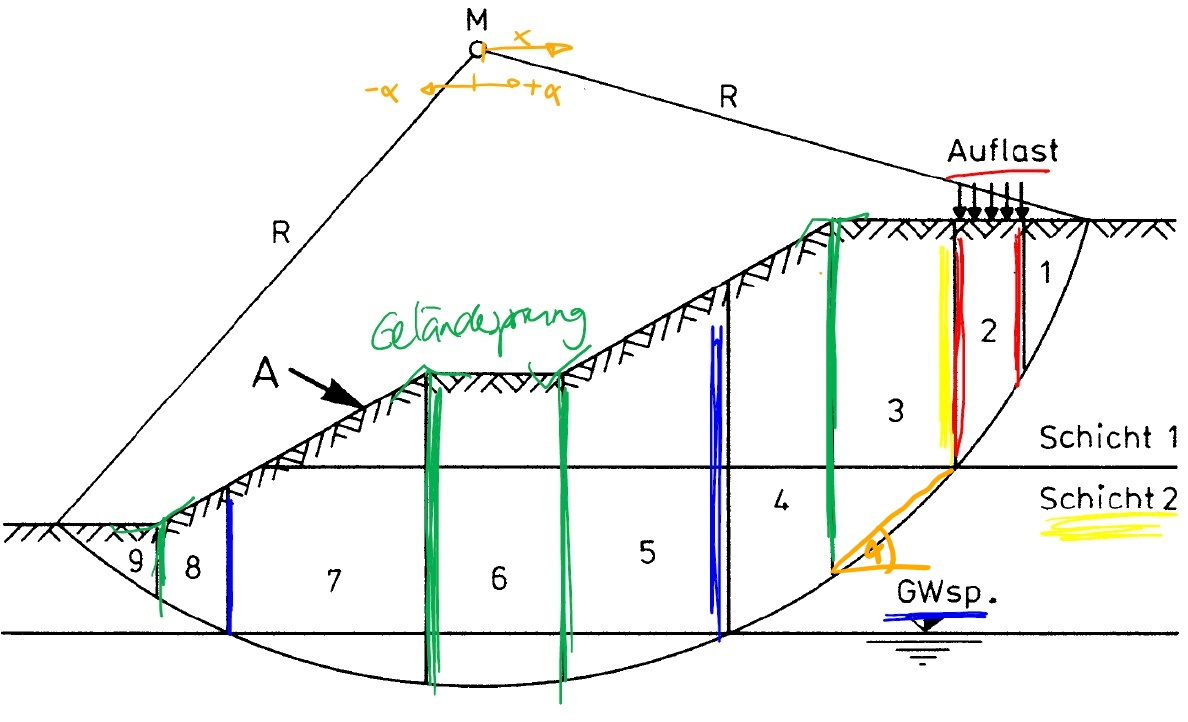
\includegraphics[width=\linewidth]{images/Boschstab1Lamelle.jpg} \\
% \end{minipage}
% \begin{minipage}{\linewidth}
		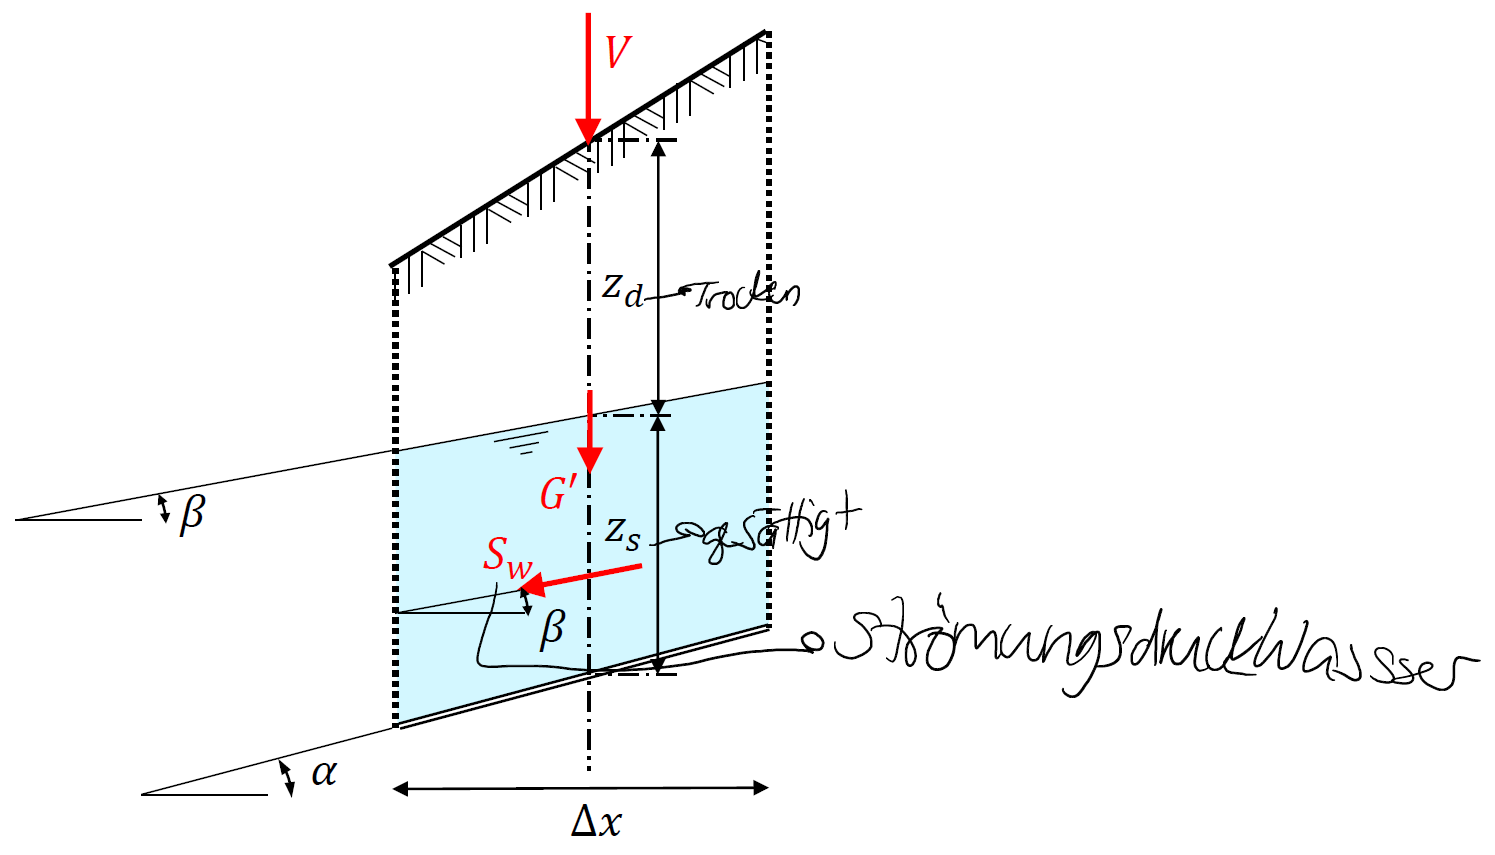
\includegraphics[width=\linewidth]{images/Boschstab2Krafte.PNG} \\
	\end{minipage}
\begin{minipage}{\linewidth}
	
	\begin{align*}		
		G' 	&= ( \gamma \cdot z_d + \gamma' \cdot z_s ) \Delta x  \\
		S_w	&= \gamma_w \cdot \Delta x \cdot sin(\beta) \cdot z_s \\
		M_E	&= G' \cdot sin(\alpha) + S_w \cdot cos(\alpha - \beta) \cdot R \\
		M_R	&= [G' \cdot sin(\alpha) - S_w \cdot sin(\alpha - \beta) ] \cdot tan(\varphi')R + c' \frac{\Delta x}{cos(\alpha)} R
	\end{align*}

\end{minipage}
\begin{minipage}{\linewidth}
	
	\begin{tabular}{l|l|l|l|l|l|l|l|l|l|l|l|l|l|l}
				& $ \Delta $ x	& (x)	& $ \alpha $	& $ \beta $	& c'	& $ \varphi' $	& $ \gamma $	& $ \gamma' $	& z$_d$	& z$_s$	& G'	& S$_w$	&	M$_E$	& M$_R$	\\ \hline
			
			Nr	& m	& m	& °	& °	& kPa	& °	& $ \frac{kN}{m^3} $	& $ \frac{kN}{m^3} $	& m	& m	& $ \frac{kN}{m} $	& $ \frac{kN}{m} $	& $ \frac{kN}{m} $	& $ \frac{kN}{m} $ \\ \hline
			
			1 &&&&&&&&&&&&&& \\
			2 &&&&&&&&&&&&&& \\
			3 &&&&&&&&&&&&&& \\
			... &&&&&&&&&&&&&& \\ \hline
			&&&&&&&&&&&&& $  \sum M_E $ & $  \sum M_R $ \\
			&&&&&&&&&&&&& \multicolumn{2}{c|}{$ F = \frac{M_R}{M_E}$} \\
	\end{tabular}

\end{minipage}